This chapter introduces and reviews general concepts of the wastewater treatment, machine learning techniques for regression.

\section{Wastewater Treatment}
\label{s:First-Background-Topic}

Provide background information that will help potential readers to understand your research. It is up to you to decide the volume and content of this chapter.



\section{Machine Learning}
\label{s:Second-Background-Topic}

\ac{ML} is an area of the \ac{AI} where a computer is programmed to learn form data \cite{Ray2019}. In 1959 Arthur Samuel defined the Machine Learning as \textbf{the field of study that gives the computers the ability to learn without being explicitly programmed}. Almost 40 years later, Tom Mitchell described Machine Learning as follows: \textbf{A computer program is said to learn from experience E with respect to some task T and some performance measure P, if its performance on T, as measured by P, improves with experience E.} \autoref{f:AI} shows the how the \ac{ML} fits in the \ac{AI} world and presents \ac{DL} as part of \ac{ML} which is presented in \autoref{s:Second-Background-Deep-Learning}.

\begin{figure}[h]
\centering
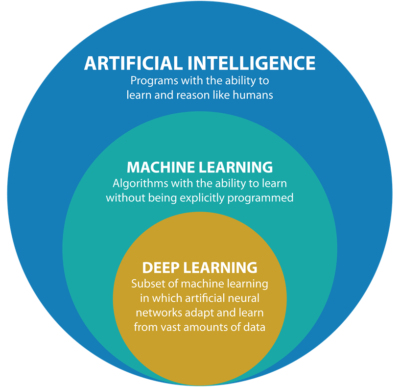
\includegraphics[width=8cm]{figures/Ch2/AI-ML-DL.png}
\caption{AI, ML, and DL \cite{raza_cinquergrana_2018}}
\label{f:AI}
\end{figure}

\begin{figure}[t]
\centering
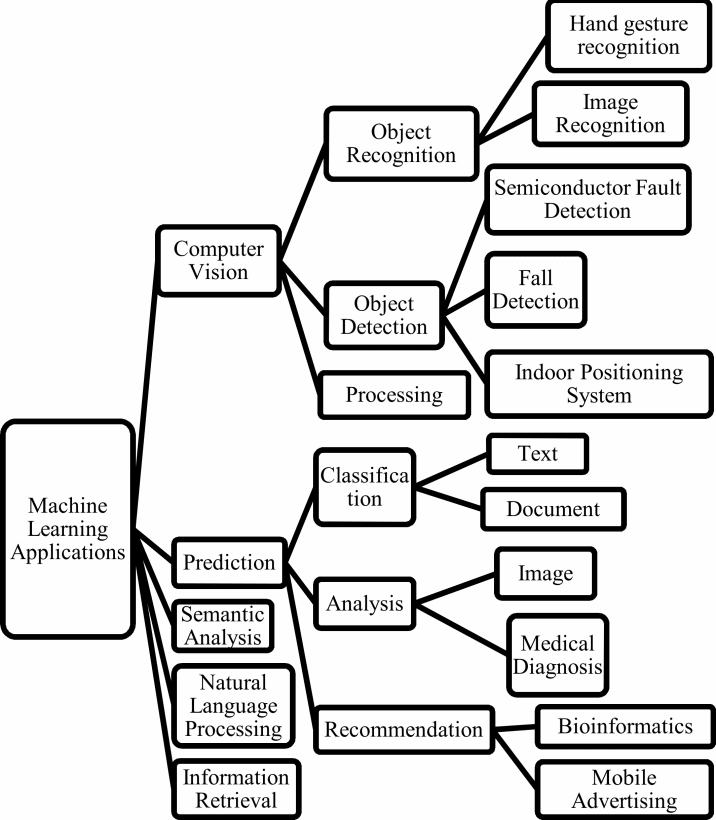
\includegraphics[width=8cm]{figures/Ch2/ML-Applications.png}
\caption{ML Applications \cite{Shinde_2018}}
\label{f:Ml-app}
\end{figure}

Now a days machine Learning is used in a variety of fields such as: robotics, biology, social science, virtual personal assistants, computer games, autonomous driving, pattern recognition, natural language processing, computer vision, product recommendation, market prediction, medical diagnosis, fraud detection, agriculture advisory, Bots, climatology, social media services, among others \cite{Srivastava_2019, Shinde_2018, Ray2019}, \autoref{f:Ml-app} shows some of the \ac{ML} application domains. 

\begin{figure}[h]
\centering
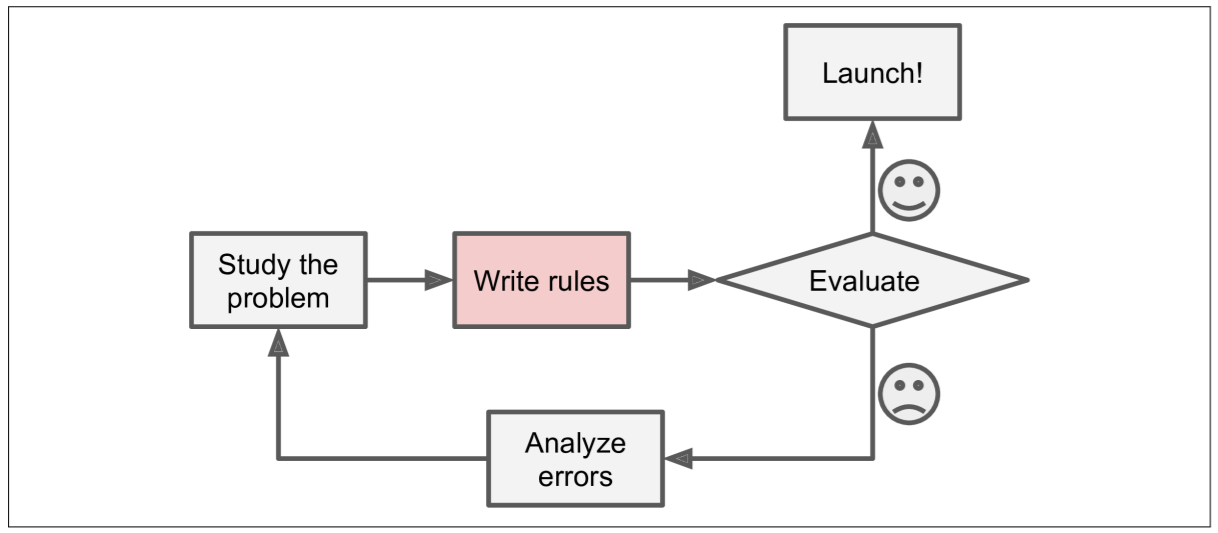
\includegraphics[width=\linewidth]{figures/Ch2/Tradicional-Approach.png}
\caption{Traditional rule based approach \cite{geron2017}}
\label{f:Traditional-approach}
\end{figure}

An important milestone was the transition from rule based programming to programs that learn automatically based on experience by the use of data. \autoref{f:Traditional-approach} shows how the rule based approach works, it starts by studying the problem, identifying some patterns and building a set of rules based on them. Subsequently, the system is evaluated and the rules are adjusted continuously in an iterative process until a good enough performance is achieved \cite{geron2017}. Should be noted that the bigger the problem the more complex the rules and more difficult the pattern identification task becomes. Meanwhile, \ac{ML} programs improve their performance during the training phase, usually presenting shorter programs, more maintainable, and more accurate. Some studies that compare the results of these data analysis methods evidence that the first tends to provide stronger scientifically sounder information, statistical assessment and uncertainty estimations, but the latter tends to bring forward better accuracy in the majority of works \cite{geron2017,Ye2020}. \autoref{f:ML-approach} illustrates the \ac{ML} approach to solve problems.

\begin{figure}[h]
\centering
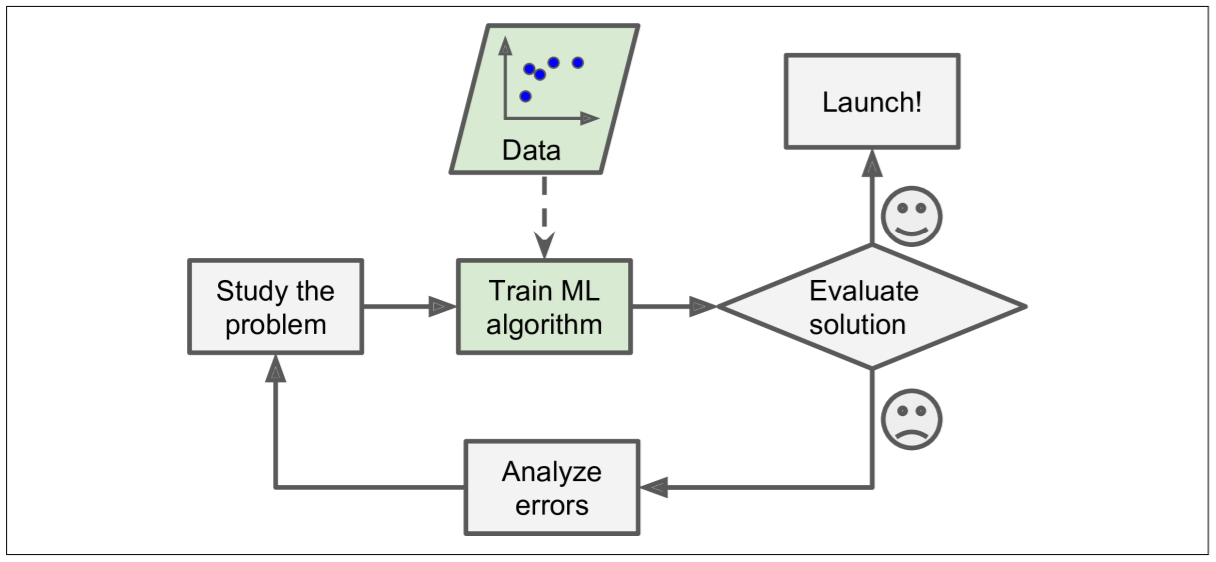
\includegraphics[width=\linewidth]{figures/Ch2/Ml-Approach.png}
\caption{ML approach \cite{geron2017}}
\label{f:ML-approach}
\end{figure}

There are different types of \ac{ML} systems, and they can be classified based on human supervision as supervised learning, unsupervised learning and reinforcement learning. 

\subsection{Supervised Learning}
This category of \ac{ML} algorithms aim to find a function capable of represent the relationship between the input and output variables from a given set of data. It is called supervised since it infers the function from labelled examples during the training stage, which means that for each input sample there is an associated and known output sample assigned by a human supervisor \cite{Batta2020}. 

\begin{figure}[h]
\centering
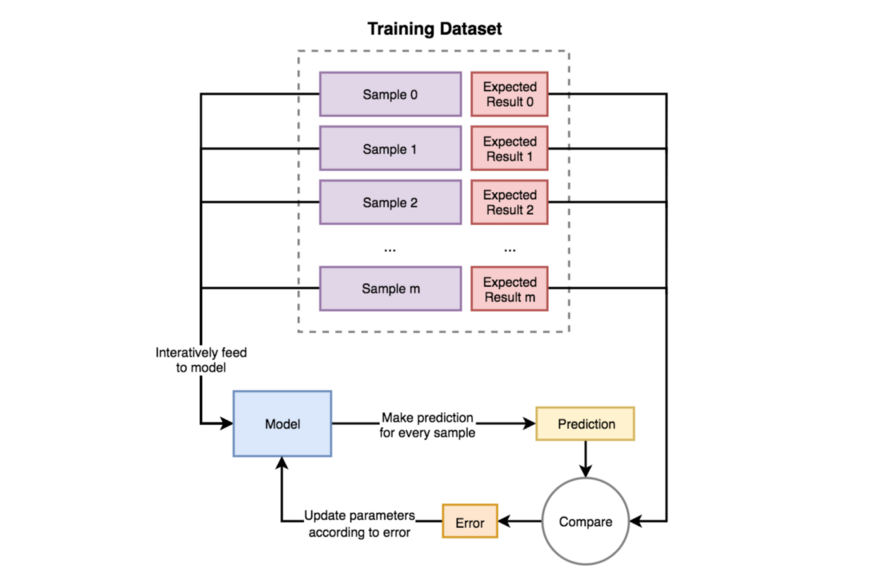
\includegraphics[width=\linewidth]{figures/Ch2/Supervised-Learning.png}
\caption{Supervised Learning}
\label{f:supervised-learning}
\end{figure}

This type of machine learning is used for both regression and classification tasks.

\begin{figure}[h]
\centering
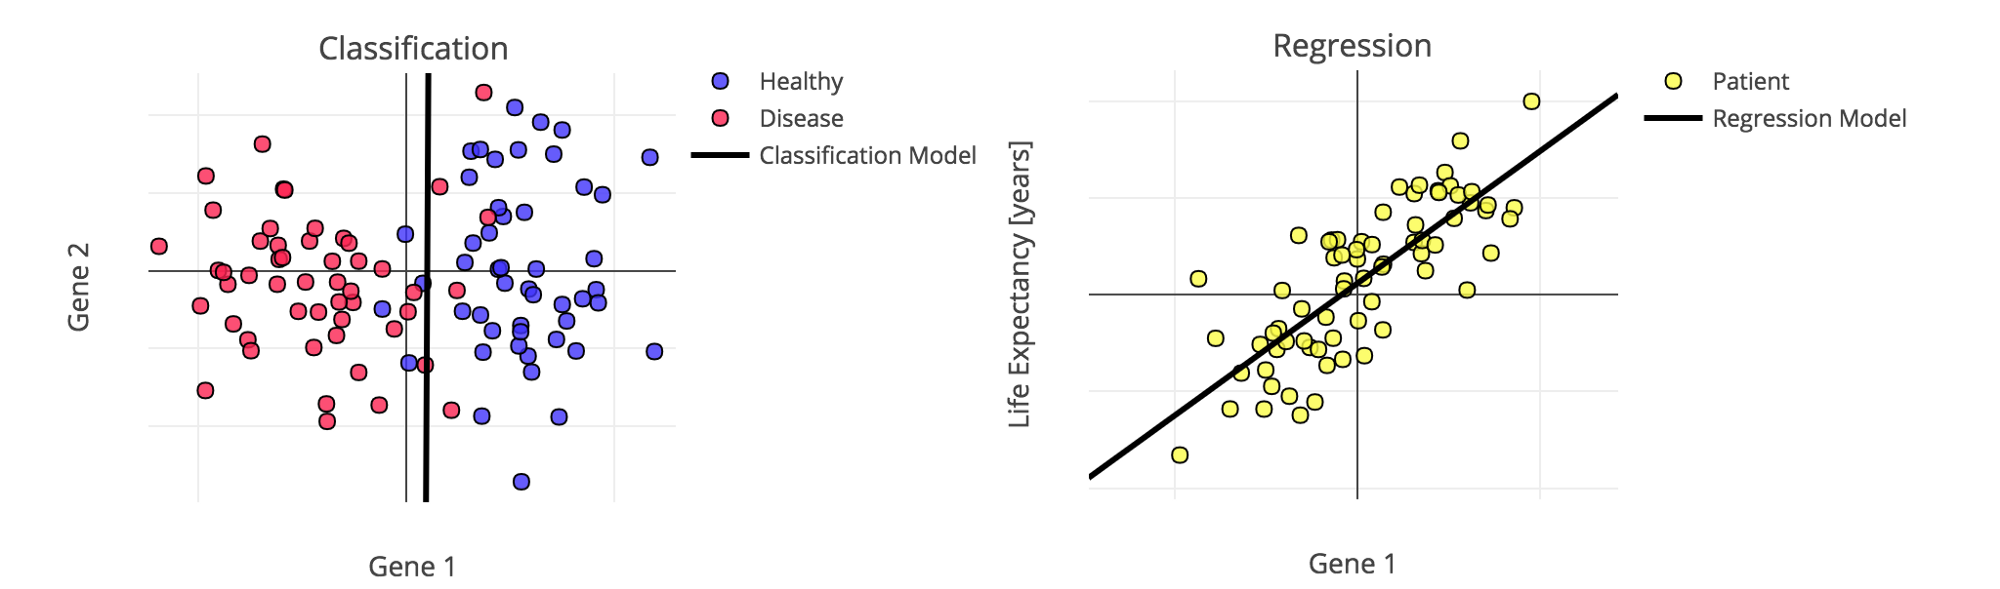
\includegraphics[width=\linewidth]{figures/Ch2/Regression-Classification.png}
\caption{Classification and Regression examples}
\label{f:classification-regression}
\end{figure}

\subsubsection{Linear Regression}
\subsubsection{Decision Tree}
\subsubsection{Support Vector Machines}

\subsection{Unsupervised Learning}
\subsubsection{PCA}
\subsubsection{Clustering}


\section{Deep Learning}
\label{s:Second-Background-Deep-Learning}

\begin{figure}[h]
\centering
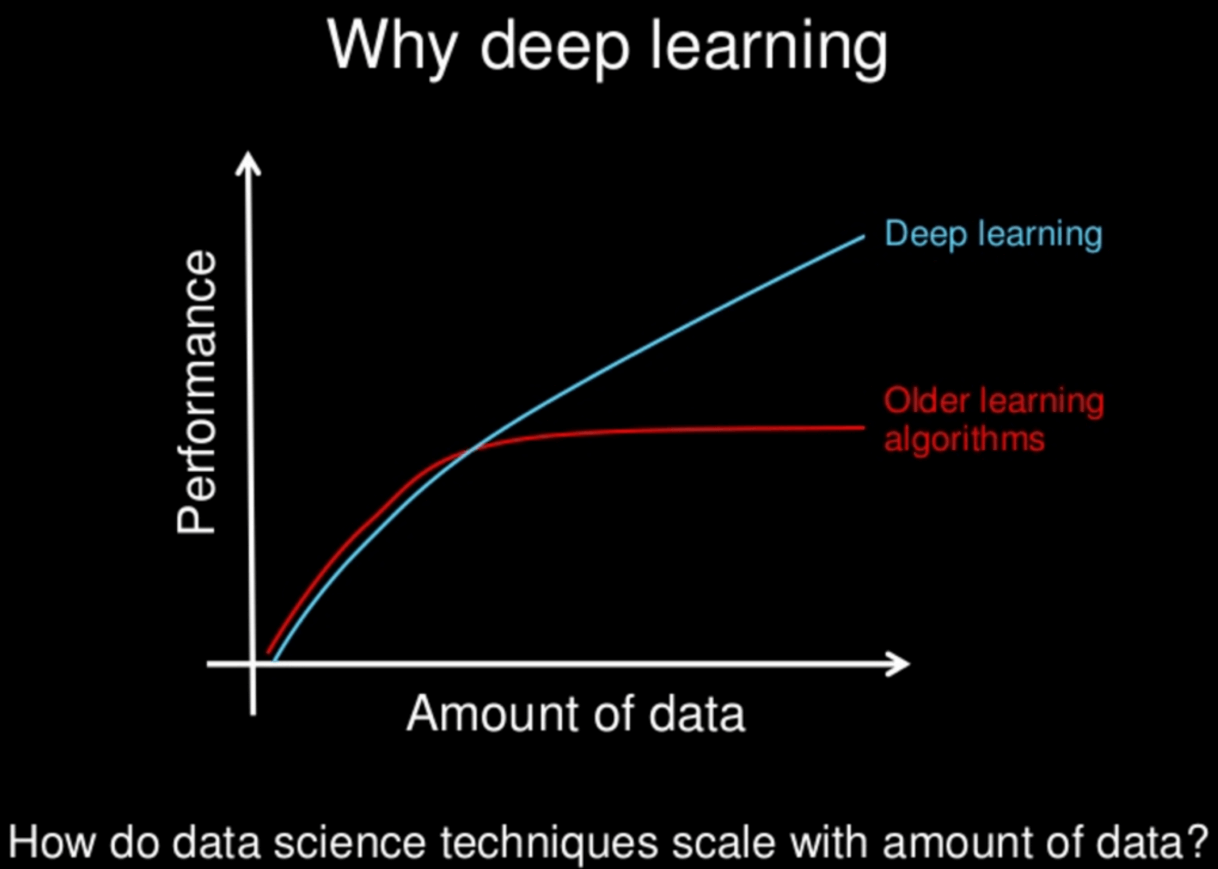
\includegraphics[width=8cm]{figures/Ch2/MlvsDL-data-amount.png}
\caption{ML vs DL}
\label{f:ML-vs-DL}
\end{figure}

\section{Evaluation Metrics}
\label{sec:section_Example}
\subsection{Mean Absolute Percentage Error}
\subsubsection{Determination Coefficient}

\section{Summary}
\label{s:Background-Summary}

The final section of each chapter should summarize the chapter. In comparison to the chapter.

